\documentclass[conference]{IEEEtran}

\let\showhyphens\relax
\usepackage{hyphenat}
\usepackage[utf8]{inputenc}
\usepackage[T1]{fontenc}
\usepackage{cite}
\usepackage{graphicx}
\usepackage{array}
\usepackage{tabularx}
\usepackage{booktabs}
\usepackage{url}
\usepackage[hidelinks]{hyperref}
\usepackage{tikz}
\usetikzlibrary{arrows.meta, positioning, fit, shapes.misc}
\usepackage{listings}
\usepackage{xcolor}
\usepackage{microtype}
\usepackage{enumitem}
\urlstyle{same}
\raggedbottom
\setlength{\emergencystretch}{2em}
\hbadness=10000
\hfuzz=10pt

\lstdefinestyle{code}{
  basicstyle=\scriptsize\ttfamily,
  breaklines=true,
  frame=single,
  columns=fullflexible,
  keepspaces=true,
  showstringspaces=false,
  xleftmargin=1mm,
  xrightmargin=1mm
}

\begin{document}
\hfuzz=10pt
\hbadness=10000
\setlist[itemize]{leftmargin=*, itemsep=1pt, topsep=2pt}
\setlist[enumerate]{leftmargin=*, itemsep=1pt, topsep=2pt}

\title{Cloud Rehosting for Cross-Platform Access to a Native Windows Desktop Application: A Case Study of GAMA Animation Engine}

\author{
\IEEEauthorblockN{Axelle Chandra, Muhammad Dafa 'Izzul Iman A., Muhammad Dhiwaul Akbar,\\
Dhimas Early Oceandy, Hammam Muhammad Yazid}
\IEEEauthorblockA{Department of Computer Science and Electronics\\
Faculty of Mathematics and Natural Sciences, Universitas Gadjah Mada\\
Yogyakarta, Indonesia}
}

\maketitle

\begin{abstract}
GAMA Animation Engine (GAE), a core component of Gamatutor, is a native Windows desktop application used to create and play simple tutorial animations. Its desktop-based architecture creates accessibility limitations because users normally need a compatible Windows environment and local installation before they can use the application. This project addresses that problem by rehosting GAE in a cloud-based environment and exposing it through browser-based remote access. The implemented architecture uses Amazon Elastic Compute Cloud (EC2) with two virtual machines: a Linux EC2 instance running Apache Guacamole as an HTML5 remote desktop gateway and a Windows EC2 instance running the GAE application. Users access the system through a web browser, while Apache Guacamole translates the browser session into an RDP connection to the Windows server. The result shows that GAE can be used from different operating systems without local installation and without significant modification to the original application source code. Although the solution is not a full cloud-native redesign, it successfully improves accessibility, simplifies user access, and demonstrates that rehosting is a practical migration approach for native Windows desktop applications that need cross-platform browser-based availability.
\end{abstract}

\begin{IEEEkeywords}
cloud computing, rehosting, legacy application, Apache Guacamole, AWS EC2, Remote Desktop Protocol, cross-platform access, GAMA Animation Engine
\end{IEEEkeywords}

\section{Introduction}

Cloud computing enables software to be accessed without depending entirely on local hardware and local installation. However, many useful applications are still designed as native desktop applications, especially older academic or institutional software that was originally built for a specific operating system. GAMA Animation Engine (GAE), part of the Gamatutor project, is one example. The original application is a Windows desktop application that includes tools such as TutorialGenerator and PlayerAnimasi for creating and playing tutorial animation content.

The main problem addressed in this project is not the absence of application functionality, but limited accessibility. In its original form, GAE is easier to use when the user has a compatible Windows device and performs local application setup. This creates barriers for users who use macOS, Linux, Chromebook, or other devices that do not directly run Windows desktop applications. It also makes the application less convenient because every user device needs its own installation and environment configuration.

This project therefore focuses on improving accessibility for a native Windows desktop application. Instead of rewriting GAE into a web application, the project keeps the original application behavior and moves the execution environment to the cloud. Users only need a browser, while the application runs on a Windows server in the cloud. This approach supports cross-platform usage and reduces local installation requirements.

The objective of this project is to design, implement, and evaluate a cloud rehosting architecture that allows GAE to be accessed through a browser. The final system uses Apache Guacamole as a web-based remote access gateway and AWS EC2 as the cloud infrastructure. The project also documents the deployment process, the weekly progress, and the use of AI assistance in preparing the final deliverables.

\section{Methods}

\subsection{Application and Problem Analysis}

GAE is treated as a native Windows desktop application. Based on the initial project analysis, the application is built using Delphi/Object Pascal with the Visual Component Library (VCL), runs as a standalone Windows application, and depends on local files such as animation files, images, and audio assets. These characteristics make the application strongly tied to the Windows desktop environment.

The accessibility problem can be summarized as follows. First, users need a compatible Windows environment to run the application directly. Second, the application must be installed or prepared on each local device. Third, users on non-Windows operating systems face additional barriers. Fourth, the local deployment model does not provide a simple centralized access point. Therefore, the project requires a deployment model that preserves the original Windows application while making it available through a universal interface: the web browser.

\subsection{Migration Strategy}

The selected migration strategy is rehosting, also known as lift-and-shift. Rehosting moves the application execution environment to cloud infrastructure with minimal changes to the original application. This strategy is appropriate for this project because the goal is to improve access rather than redesign the software architecture.

Alternative approaches such as rewriting GAE as a web application or converting it into a fully cloud-native system would require a much larger engineering effort. Those approaches could also change the behavior of the existing application. Rehosting was selected because it can preserve the Windows desktop execution environment while allowing users to access the application remotely.

\subsection{Target Architecture}

The target architecture consists of three layers: the client layer, the gateway layer, and the target application layer. The client layer is the user's device and web browser. The gateway layer is a Linux EC2 instance running Apache Guacamole. The target application layer is a Windows EC2 instance that runs GAE. The browser connects to Guacamole through HTTP on port 8080 during the prototype stage. Guacamole then connects to the Windows EC2 instance through Remote Desktop Protocol (RDP) on port 3389.

Apache Guacamole was selected because it allows users to access remote desktops from a web browser. The Guacamole web application communicates with \texttt{guacd}, the native Guacamole proxy, which then connects to remote desktop servers. Guacamole supports protocol translation so that the browser-side client does not need to understand RDP directly \cite{apacheguac}. AWS EC2 was selected as the infrastructure provider because EC2 provides virtual servers with configurable compute, networking, and storage resources \cite{awsec2}.

\begin{figure*}[!t]
\centering
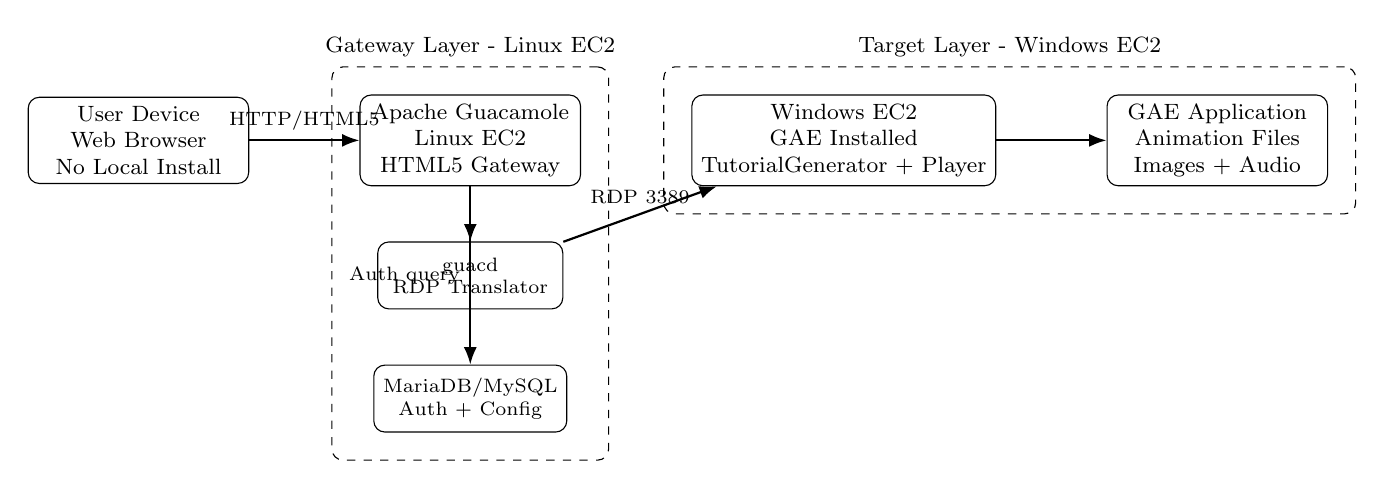
\begin{tikzpicture}[
  node distance=1.15cm and 1.4cm,
  box/.style={draw, rounded corners, align=center, minimum height=1cm, minimum width=2.8cm, font=\footnotesize},
  smallbox/.style={draw, rounded corners, align=center, minimum height=0.85cm, minimum width=2.35cm, font=\scriptsize},
  arrow/.style={-{Latex[length=2.2mm]}, thick},
  group/.style={draw, rounded corners, dashed, inner sep=0.35cm}
]

\node[box] (user) {User Device\\Web Browser\\No Local Install};
\node[box, right=of user] (guac) {Apache Guacamole\\Linux EC2\\HTML5 Gateway};
\node[smallbox, below=0.7cm of guac] (guacd) {guacd\\RDP Translator};
\node[smallbox, below=0.7cm of guacd] (db) {MariaDB/MySQL\\Auth + Config};
\node[box, right=of guac] (win) {Windows EC2\\GAE Installed\\TutorialGenerator + Player};
\node[box, right=of win] (gae) {GAE Application\\Animation Files\\Images + Audio};

\draw[arrow] (user) -- node[above, font=\scriptsize]{HTTP/HTML5} (guac);
\draw[arrow] (guac) -- (guacd);
\draw[arrow] (guacd) -- node[above, font=\scriptsize]{RDP 3389} (win);
\draw[arrow] (win) -- (gae);
\draw[arrow] (guac) -- node[left, font=\scriptsize]{Auth query} (db);

\node[group, fit=(guac)(guacd)(db), label={[font=\footnotesize]above:Gateway Layer - Linux EC2}] {};
\node[group, fit=(win)(gae), label={[font=\footnotesize]above:Target Layer - Windows EC2}] {};

\end{tikzpicture}
\caption{Target cloud rehosting architecture for browser-based access to GAE.}
\label{fig:architecture}
\end{figure*}

\subsection{Infrastructure Components}

Table \ref{tab:components} summarizes the main infrastructure components used in the project. The architecture separates user access from the Windows application host. This separation allows the Windows instance to be protected from direct public exposure while the Guacamole gateway becomes the browser-facing access point.

\begin{table}[!t]
\centering
\caption{Infrastructure Components}
\label{tab:components}
\small
\begin{tabular}{@{}>{\raggedright\arraybackslash}p{2.05cm}>{\raggedright\arraybackslash}p{5.05cm}@{}}
\toprule
\textbf{Component} & \textbf{Role} \\
\midrule
User browser & Accesses GAE without local installation. \\
Linux EC2 & Hosts the Apache Guacamole gateway. \\
Apache Guacamole & Provides browser-based remote desktop access. \\
\texttt{guacd} & Translates the Guacamole protocol to RDP. \\
MariaDB/\linebreak MySQL & Stores Guacamole users, connections, and configuration. \\
Windows EC2 & Runs the original GAE desktop application. \\
RDP & Connects Guacamole to the Windows desktop environment. \\
\bottomrule
\end{tabular}
\end{table}

\subsection{Deployment Procedure}

The deployment process was divided into local proof-of-concept testing and cloud implementation. The local proof of concept was used to verify that the application could run inside a virtualized Windows environment and could be accessed through RDP. After that, the cloud infrastructure was prepared on AWS.

The cloud deployment process consists of the following steps:

\begin{enumerate}
    \item Prepare an AWS account and configure a project budget to control cost.
    \item Create a Virtual Private Cloud (VPC), subnet, route table, and internet gateway.
    \item Launch a Linux EC2 instance to host Apache Guacamole.
    \item Launch a Windows EC2 instance to run the GAE application.
    \item Configure security groups so that browser users access Guacamole through port 8080, while RDP access to Windows is limited to the internal VPC or the Guacamole gateway.
    \item Install Docker and Docker Compose on the Linux EC2 instance.
    \item Deploy Guacamole, \texttt{guacd}, and database services using the deployment repository.
    \item Install GAE on the Windows EC2 instance using the original Gamatutor application artifact.
    \item Create a Guacamole RDP connection pointing to the private address of the Windows EC2 instance.
    \item Test the system from a browser and compare the behavior with the local environment.
\end{enumerate}

\subsection{Repositories}

Two repositories are used in this project. The first repository is the original Gamatutor/GAE application repository. It is treated as the application artifact that is rehosted to the Windows EC2 instance \cite{gamatutor}. The second repository is the deployment configuration repository created for this cloud computing project. It contains Docker-related configuration files for preparing the Guacamole gateway layer \cite{deploymentrepo}.

This separation is important. The project does not claim to rewrite or rebuild GAE. Instead, it rehosts the existing application and uses a separate deployment configuration to make the application accessible through a browser.

\section{Results}

\subsection{Local Proof of Concept}

The first milestone was a local proof of concept using a virtual machine. The team created a local VM using VirtualBox, installed the application inside the VM, and successfully accessed it through RDP. At that stage, Guacamole installation and integration were still unresolved, and the project progress was reported as 40\%. This proof of concept was important because it verified that GAE can be executed from a virtualized Windows environment and accessed remotely before moving the setup to cloud infrastructure.

\subsection{Cloud Rehosting Result}

The final cloud implementation successfully rehosted GAE using the architecture shown in Fig. \ref{fig:architecture}. The user accesses the system from a browser, the request is handled by Apache Guacamole running on Linux EC2, and the GAE desktop environment is delivered from a Windows EC2 instance through RDP. The team reported the final progress as 100\% after the cloud access architecture was completed.

The final implementation achieved the main accessibility goals. First, users no longer need to install GAE on their local devices. Second, users from different operating systems can access the application as long as they have a compatible web browser. Third, the original GAE application can continue running in its Windows environment. Fourth, the deployment provides a centralized access point through Guacamole.

\subsection{Functional Testing}

Table \ref{tab:functional} presents the functional test summary. The test cases focus on accessibility and basic application operation rather than performance benchmarking, because the project goal is to validate the feasibility of browser-based rehosting.

\begin{table}[!t]
\centering
\caption{Functional Testing Summary}
\label{tab:functional}
\scriptsize
\begin{tabular}{@{}>{\raggedright\arraybackslash}p{0.4cm}>{\raggedright\arraybackslash}p{5.35cm}>{\centering\arraybackslash}p{1.05cm}@{}}
\toprule
\textbf{No.} & \textbf{Test Case} & \textbf{Status} \\
\midrule
1 & Run GAE in local Windows environment. & Passed \\
2 & Access virtualized Windows environment through RDP. & Passed \\
3 & Deploy Guacamole gateway on Linux EC2. & Passed \\
4 & Connect Guacamole to Windows EC2 through RDP. & Passed \\
5 & Access Windows EC2 from a browser through Guacamole. & Passed \\
6 & Run GAE on the Windows EC2 instance. & Passed \\
7 & Use browser-only access without installing GAE locally. & Passed \\
\bottomrule
\end{tabular}
\end{table}

\subsection{Deployment Configuration Result}

The deployment repository uses Docker Compose to define the Guacamole gateway environment. The main services include Guacamole, \texttt{guacd}, and a MariaDB/MySQL database. The Guacamole service exposes port 8080 during the prototype stage, while \texttt{guacd} handles remote desktop protocol translation. The database stores authentication data and connection configuration.

The use of Docker Compose simplified the gateway setup because the required services could be started consistently on the Linux EC2 instance. However, the prototype configuration also revealed security concerns, such as the use of simple credentials and hardcoded secrets in configuration files. These issues are discussed as limitations in Section \ref{sec:discussion}.

\subsection{Video Demonstration Attachments}

The final deliverables require two video demonstrations. The first video demonstrates GAE running in the local or on-premise environment. The second video demonstrates GAE running through the cloud server using browser-based access via Guacamole. These videos should be submitted as separate attachments or linked in the appendix.

\section{Discussion}
\label{sec:discussion}

\subsection{Accessibility Improvement}

The main value of the project is improved accessibility. In the original model, users need a Windows-compatible local environment. In the rehosted model, users only need a browser. The actual Windows execution environment is moved to the cloud, while Guacamole presents the remote session through an HTML5 web interface.

This design directly addresses cross-platform access. A user on Windows, macOS, Linux, or another device with a modern browser can access the same application environment. The approach also reduces local setup complexity because users do not need to install GAE and its dependencies on each device.

\subsection{Why Rehosting is Suitable}

Rehosting is suitable because it solves the accessibility problem without changing the core application. The original GAE behavior is preserved because the application still runs inside a Windows desktop environment. At the same time, cloud infrastructure provides centralized access and reduces device-level dependency.

This is different from making the application cloud-native. A cloud-native redesign would require major changes such as rewriting the UI for the web, redesigning file handling, and possibly building a server-side architecture. Those changes are outside the scope of this project. The selected approach is therefore more realistic for a cloud computing final project focused on legacy application rehosting.

\subsection{Security Considerations}

Security is a critical consideration because remote desktop access can expose sensitive infrastructure if it is misconfigured. The Windows EC2 instance should not expose RDP directly to the public internet. Instead, RDP should be restricted to the Guacamole gateway inside the VPC. The Guacamole interface should also use HTTPS in a production environment. Strong passwords, limited inbound rules, and periodic credential rotation are recommended.

The prototype deployment configuration also uses hardcoded credentials and secret values. This is acceptable only as a temporary classroom prototype. In a production setup, secrets should be moved to environment variables, a private configuration file excluded from Git, or a secret management service. The default Guacamole account should also be changed immediately after installation.

\subsection{Operational Limitations}

The solution still depends on a Windows EC2 instance. Therefore, operating cost is higher than a purely static web application and the system must be managed like a remote desktop environment. Performance also depends on network quality, browser responsiveness, and RDP session stability. For multi-user use, the team must consider Windows licensing, concurrent session limits, user isolation, and storage management.

Another limitation is that this prototype focuses on access and feasibility rather than extensive performance evaluation. No detailed latency benchmark, bandwidth benchmark, or concurrent-user stress test was performed. Future work should include those measurements to evaluate the system under more realistic user loads.

\subsection{Future Improvements}

Several improvements can make the system more production-ready. First, HTTPS should be configured using a domain and TLS certificate. Second, authentication should be strengthened using unique accounts and possibly multi-factor authentication. Third, RDP access should be restricted through private networking and security group references. Fourth, backups should be configured for animation files and Guacamole configuration. Fifth, cloud cost can be reduced by stopping instances when they are not used or scheduling runtime based on class usage.

\section{Conclusion}

This project successfully improved the accessibility of GAE, a native Windows desktop application, by rehosting it in a cloud environment. The implemented architecture uses a Linux EC2 instance running Apache Guacamole as a browser-based gateway and a Windows EC2 instance as the application host. Through this architecture, users can access GAE from different operating systems without installing the application locally.

The result demonstrates that rehosting is a practical approach for making Windows desktop applications accessible through a browser while preserving the original application behavior. Although the system is not a complete cloud-native redesign, it satisfies the main project objective: solving the accessibility limitation of a Windows-native desktop application through cloud-based, cross-platform, browser-only access.

\begin{thebibliography}{00}

\bibitem{ieeetemplate} IEEE, ``IEEE Conference Templates,'' IEEE Author Center. [Online]. Available: \url{https://www.ieee.org/conferences/publishing/templates}

\bibitem{imrad} T. Dube, ``IMRAD In Science: The Importance a Format Can Have,'' \textit{Medium}, Dec. 7, 2015. [Online]. Available: \url{https://medium.com/literacy-discourse/imrad-in-science-4a29e6c63ccc}

\bibitem{awsec2} Amazon Web Services, ``What is Amazon EC2?,'' \textit{Amazon Elastic Compute Cloud User Guide}. [Online]. Available: \url{https://docs.aws.amazon.com/AWSEC2/latest/UserGuide/concepts.html}

\bibitem{apacheguac} Apache Software Foundation, ``Implementation and architecture,'' \textit{Apache Guacamole Manual}. [Online]. Available: \url{https://guacamole.apache.org/doc/gug/guacamole-architecture.html}

\bibitem{guacdocker} Apache Software Foundation, ``Containerized (Docker) installation,'' \textit{Apache Guacamole Manual}. [Online]. Available: \url{https://guacamole.apache.org/doc/gug/guacamole-docker.html}

\bibitem{dockercompose} Docker Inc., ``Docker Compose overview,'' \textit{Docker Documentation}. [Online]. Available: \url{https://docs.docker.com/compose/}

\bibitem{gamatutor} Gamatutor, ``gamatutor/gamatutor: GAE - Engine Pembuat dan Player Animasi Tutorial Sederhana,'' GitHub. [Online]. Available: \url{https://github.com/gamatutor/gamatutor}

\bibitem{deploymentrepo} EarlyOcean, ``cloud-computing-final-project,'' GitHub. [Online]. Available: \url{https://github.com/EarlyOcean/cloud-computing-final-project}

\bibitem{rdp} Microsoft, ``Remote Desktop Services,'' Microsoft Learn. [Online]. Available: \url{https://learn.microsoft.com/en-us/windows-server/remote/remote-desktop-services/}

\end{thebibliography}

\clearpage
\onecolumn
\appendices

\section{Weekly Progress Submitted to Simaster}

Table \ref{tab:weekly} summarizes the weekly progress based on the project plan and submitted progress reports. Each progress presentation files from week 3 on can be accessed via this link: \url{https://drive.google.com/drive/folders/1_TIOAsoQKRpXNc5k8S584nojheTPT_be?usp=sharing}.

\begin{table}[!htbp]
\centering
\small
\caption{Weekly Progress Summary}
\label{tab:weekly}
\begin{tabularx}{\textwidth}{p{1.2cm}p{4.2cm}X p{2.2cm}}
\toprule
\textbf{Week} & \textbf{Main Activity} & \textbf{Output} & \textbf{Status} \\
\midrule
1 & Problem identification and application analysis & Identified GAE as a Windows-native desktop application with accessibility limitations and local installation dependency. & Completed \\
2 & Migration strategy selection & Selected rehosting/lift-and-shift as the most suitable approach for preserving the original application while improving access. & Completed \\
3 & Initial cloud architecture design & Designed an architecture using a gateway layer and a Windows application host. & Completed \\
4 & Local proof of concept & Created a local VM using VirtualBox, installed the application, and accessed it through RDP. Guacamole integration was still in progress. & 40\% progress \\
5 & AWS setup and EC2 provisioning & Prepared AWS budget, VPC, Linux EC2, and Windows EC2 instances for cloud implementation. & Completed \\
6 & Guacamole deployment and integration & Deployed Apache Guacamole, \texttt{guacd}, and database services on Linux EC2 and connected them to Windows EC2. & Completed \\
7 & Final testing, documentation, and demonstration & Verified browser-based access to GAE through Guacamole and prepared final report, appendix, and video demonstrations. & 100\% progress \\
\bottomrule
\end{tabularx}
\end{table}

\section{Step-by-Step Documentation}

This appendix describes the rehosting procedure used in the project. The exact values for instance IDs, passwords, private keys, and IP addresses should be adjusted according to the active deployment environment.

\subsection{Prepare AWS Budget and Network}

Create an AWS budget to limit unexpected usage cost. Then create a VPC for the project. The VPC should contain at least one public subnet for the Guacamole gateway and a route table connected to an internet gateway. The Windows instance can be placed in the same VPC and should receive private connectivity from the Guacamole gateway.

\subsection{Launch Linux EC2 for Guacamole}

Launch an Ubuntu Linux EC2 instance. Attach a security group that allows SSH from the administrator's IP address and HTTP access to the Guacamole prototype port. In a production configuration, port 8080 should be placed behind HTTPS using a reverse proxy.

\begin{lstlisting}[style=code,caption={Example Linux EC2 access command}]
ssh -i /path/to/keypair.pem ubuntu@<linux-ec2-public-ip>
\end{lstlisting}

\subsection{Install Docker and Docker Compose}

Install Docker and Docker Compose on the Linux EC2 instance. The exact commands may vary depending on the operating system image.

\begin{lstlisting}[style=code,caption={Example Docker installation commands}]
sudo apt update
sudo apt install -y docker.io docker-compose-v2
sudo systemctl enable docker
sudo systemctl start docker
sudo usermod -aG docker ubuntu
\end{lstlisting}

\subsection{Deploy Guacamole Services}

Clone the deployment repository and start the Docker Compose services. The project repository contains configuration for Guacamole, \texttt{guacd}, database, and supporting services.

\begin{lstlisting}[style=code,caption={Deploying the Guacamole gateway}]
git clone https://github.com/EarlyOcean/cloud-computing-final-project.git
cd cloud-computing-final-project
mkdir -p init data drive record
docker compose up -d
\end{lstlisting}

After the containers are running, verify the deployment.

\begin{lstlisting}[style=code,caption={Checking running containers}]
docker compose ps
\end{lstlisting}

Open the Guacamole web interface from a browser using the Linux EC2 public IP address and port 8080.

\begin{lstlisting}[style=code,caption={Prototype Guacamole URL format}]
http://<linux-ec2-public-ip>:8080/guacamole/
\end{lstlisting}

\subsection{Launch Windows EC2 for GAE}

Launch a Windows Server EC2 instance. Configure the security group so that RDP port 3389 is reachable only from the Guacamole gateway or from the internal VPC, not from the entire public internet. Retrieve the Windows administrator password using the selected key pair.

\subsection{Install GAE on Windows EC2}

Download the original Gamatutor/GAE application artifact from the official repository. Install or copy the required application files to the Windows EC2 instance. Verify that the application components such as TutorialGenerator and PlayerAnimasi can be executed in the Windows environment.

\begin{lstlisting}[style=code,caption={Original application repository}]
https://github.com/gamatutor/gamatutor
\end{lstlisting}

\subsection{Create Guacamole RDP Connection}

Log in to Guacamole as an administrator and create a new RDP connection. Configure the connection using the private IP address of the Windows EC2 instance, port 3389, and the Windows login credentials. After saving the connection, open it from the Guacamole dashboard to verify that the Windows desktop appears in the browser.

\subsection{Run GAE Through Browser}

From the browser-based Guacamole session, run the GAE application on the Windows EC2 desktop. The user should be able to interact with GAE without installing it locally. This verifies the main goal of the project: cross-platform browser-based access to a native Windows desktop application.

\section{Source Code and Deployment Repositories}

The project uses two repositories:

\begin{itemize}
    \item Original GAE/Gamatutor application repository: \url{https://github.com/gamatutor/gamatutor}
    \item Deployment configuration repository: \url{https://github.com/EarlyOcean/cloud-computing-final-project}
\end{itemize}

The original repository contains the GAE application artifact. The deployment repository contains Docker-related configuration for the remote access gateway. The original GAE source code was not significantly modified. The project focuses on rehosting the existing Windows desktop application and making it accessible through cloud infrastructure.

\section{Video Demonstration Attachments}

Two video demonstrations are included as final attachments:

\begin{itemize}
    \item \textbf{Video 1 - Local/on-premise demonstration:} shows GAE running in a local Windows environment or local VM before cloud rehosting.
    \item \textbf{Video 2 - Cloud server demonstration:} shows GAE accessed through a web browser using Apache Guacamole connected to the Windows EC2 instance.
\end{itemize}

Below we have provided both videos' URLs:

\begin{itemize}
    \item Video 1 URL: \url{https://drive.google.com/file/d/1L-oIZh7eiHuE2NPdAiUtC82iIiFoazDk/view?usp=drive_link}
    \item Video 2 URL: \url{https://drive.google.com/file/d/1URIwPxqD7alQlYP0RTKFy69g9Vzn-PHo/view?usp=drive_link}
\end{itemize}


\section{AI Declaration}

The authors used AI assistance in preparing the final deliverables. The AI product used was ChatGPT by OpenAI. AI was used as a writing and organization aid, particularly for structuring the IEEE-style report, refining the IMRAD flow, improving academic wording, organizing the appendix, and preparing the AI declaration. AI was not used as a substitute for implementation, deployment, testing, or video demonstration. The technical implementation, repository configuration, validation, and final submission decisions remain the responsibility of the authors.

The following prompt log has been cleaned and consolidated for readability while preserving the substance of the requests used during report preparation:

\begin{enumerate}
    \item ``Suggest the most suitable workflow for preparing a cloud computing final report in IEEE format using the IMRAD structure.''
    \item ``Explain whether the IEEE report can be written manually using LaTeX and provide a basic IEEE LaTeX structure.''
    \item ``Create an initial report outline for a cloud computing final project about rehosting GAE/Gamatutor, including abstract, introduction, methods, results, discussion, conclusion, references, appendix, and AI declaration.''
    \item ``Revise the project narrative so the main focus is improving accessibility for a native Windows desktop application, enabling cross-platform use, browser-only access, and no local installation.''
    \item ``Integrate the original Gamatutor application repository and the deployment configuration repository into the report as separate sources.''
    \item ``Draft an IEEE-style final report for the GAE rehosting project using Apache Guacamole, Linux EC2, Windows EC2, RDP, Docker Compose, and browser-based access.'''
\end{enumerate}

All AI-assisted text was reviewed and edited by the authors to match the actual project scope, implementation details, and final deliverable requirements.

\end{document}
